We will be looking at all the details and procedure of our analysis.

\section{Procedure}
\begin{enumerate}
    \item Start the testing apparatus by making necessary arrangements like checking pressure valve and see if inlet pressure is sufficient enough.
    \item Mount the nozzle whose pressure distribution is to be measured and
connect pressure pipes with vanes of Nozzle.
    \item First keep the inlet gauge pressure as 500 kN/m2 constant and take
reading of all pressures across nozzle by varying the exit pressure from 0 to
400 KN/m2.
    \item Then keep exit pressure as 50kN/m2 constant and take reading of all
pressures across nozzle by varying the inlet pressure.
    \item Tabulate the readings and do necessary calculations.
    \item Plot relevant graphs as mentioned.
    \item Repeat the procedures 2-6 for different nozzles given.
\end{enumerate}

\newpage
\section{Block diagram of experimental Set-up}
\begin{figure}[!h]
    \centering
    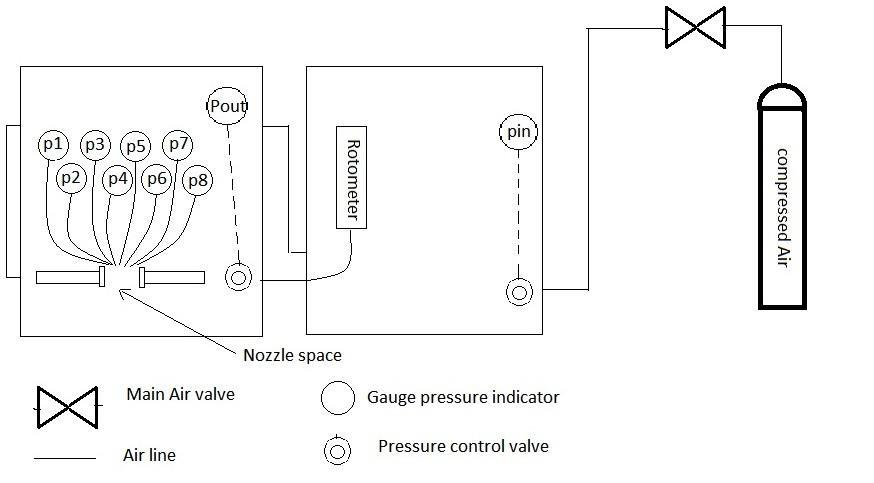
\includegraphics[width=16cm]{experimental setup.jpg}
    \caption{Experimental Setup}
\end{figure}


\section{Observation}
\[Ambient pressure = 101.325kN/m^2\]
\begin{itemize}
    \item {\Large Nozzle A}
        
{\tiny
\noindent\setlength\tabcolsep{4pt}%
\begin{tabularx}{\linewidth}{|c|c|*{10}{>{\RaggedRight\arraybackslash}X|}}
  \hline
   Pi kN/m2 & Po kN/m2 & Pressure ratio & Mass flow rate (g/s) & p1 kN/m2 & p2 kN/m2 & p3 kN/m2 & p4 kN/m2 & p5 kN/m2 & p6 kN/m2 & p7 kN/m2 & p8 kN/m2   \\
  \hline
  601.325 & 151.325 & 0.25165 & 4.4 & 541.325 & 321.325 & 221.325 & 151.325	& 111.325 & 91.325	& 101.325	& 101.325 \\
  \hline
  601.325	& 201.325	& 0.33480	& 4.4	& 541.325	& 321.325	& 221.325	& 151.325	& 111.325	& 91.325	& 101.325	& 181.325 \\
  \hline
  601.325	& 251.325	& 0.41795	& 4.4	& 541.325	& 321.325	& 221.325	& 151.325	& 111.325	& 101.325	& 221.325	& 231.325 \\
  \hline
  601.325	& 301.325	& 0.50110	& 4.4	& 541.325	& 321.325	& 221.325	& 181.325	& 241.325	& 251.325	& 281.325	& 181.325 \\
  \hline
  601.325	& 351.325	& 0.58425	& 4.4	& 541.325	& 321.325	& 221.325	& 271.325	& 281.325	& 301.325	& 331.325	& 341.325 \\
  \hline
  601.325	& 401.325	& 0.66740	& 4.4	& 541.325	& 321.325	& 231.325	& 321.325	& 331.325	& 351.325	& 381.325	& 401.325 \\
  \hline
\end{tabularx}
\captionof{table}{Constant Inlet Pressure 601.325 kN/m2}}
\vskip1cm

{\tiny
\noindent\setlength\tabcolsep{4pt}%
\begin{tabularx}{\linewidth}{|c|c|*{10}{>{\RaggedRight\arraybackslash}X|}}
  \hline
   Pi kN/m2 & Po kN/m2 & Pressure ratio & Mass flow rate (g/s) & p1 kN/m2 & p2 kN/m2 & p3 kN/m2 & p4 kN/m2 & p5 kN/m2 & p6 kN/m2 & p7 kN/m2 & p8 kN/m2   \\
  \hline
  251.325	& 151.325	& 0.60211	& 1.6	& 231.325	& 141.325	& 101.325	& 111.325	& 121.325	& 131.325	& 141.325	& 151.325 \\
  \hline
  301.325	& 151.325	& 0.50220	& 2	& 271.325	& 271.325	& 111.325 & 101.325	& 111.325	& 121.325	& 141.325	& 151.325 \\
  \hline
  351.325	& 151.325	& 0.43073	& 2.4	& 321.325	& 181.325	& 131.325	& 101.325	& 101.325	& 121.325	& 141.325	& 141.325 \\
  \hline
  401.325	& 151.325	& 0.37706	& 2.8	& 361.325	& 221.325	& 141.325	& 101.325	& 81.325	& 91.325	& 111.325	& 141.325 \\
  \hline
  451.325	& 151.325	& 0.33529	& 3.2	& 401.325	& 241.325	& 161.325	& 111.325	& 81.325	& 71.325	& 111.325	& 131.325 \\
  \hline
  501.325	& 151.325	& 0.30185	& 3.6	& 451.325	& 261.325	& 181.325	& 121.325	& 91.325	& 71.325	& 81.325	& 131.325 \\
  \hline
  551.325	& 151.325	& 0.27447	& 4	& 491.325	& 291.325	& 201.325	& 131.325	& 101.325	& 81.325	& 91.325	& 111.325 \\
  \hline
  601.325	& 151.325	& 0.25165	& 4.4	& 541.325	& 321.325	& 221.325	& 151.325	& 111.325	& 91.325	& 101.325	& 101.325 \\
  \hline
\end{tabularx}
\captionof{table}{Constant Outlet Pressure 151.325 kN/m2}}
\vskip1cm

    \item {\Large Nozzle B}

{\tiny
\noindent\setlength\tabcolsep{4pt}%
\begin{tabularx}{\linewidth}{|c|c|*{7}{>{\RaggedRight\arraybackslash}X|}}
  \hline
   Pi kN/m2 & Po kN/m2 & Pressure ratio & Mass Flow Rate (g/s) & p1 kN/m2 & p2 kN/m2 & p3 kN/m2 & p4 kN/m2 & p5 kN/m2  \\
  \hline
  601.325	& 151.325	& 0.25165	& 4.4	& 521.325	& 281.325	& 221.325	& 181.325	& 121.325 \\
  \hline
  601.325	& 201.325	& 0.33480	& 4.4	& 531.325	& 281.325	& 211.325	& 181.325	& 141.325 \\
  \hline
  601.325	& 251.325	& 0.41795	& 4.4	& 531.325	& 281.325	& 211.325	& 181.325	& 201.325 \\
  \hline
  601.325	& 301.325	& 0.50110	& 4.4	& 531.325	& 281.325	& 211.325	& 181.325	& 271.325 \\
  \hline
  601.325	& 351.325	& 0.58425	& 4.4	& 531.325	& 281.325	& 211.325	& 301.325	& 331.325 \\
  \hline
  601.325	& 401.325	& 0.66740	& 4.4	& 531.325	& 281.325	& 271.325	& 361.325	& 381.325 \\
  \hline
\end{tabularx}
\captionof{table}{Constant Inlet Pressure 601.325 kN/m2}}
\vskip1cm


{\tiny
\noindent\setlength\tabcolsep{4pt}%
\begin{tabularx}{\linewidth}{|c|c|*{7}{>{\RaggedRight\arraybackslash}X|}}
  \hline
   Pi kN/m2 & Po kN/m2 & Pressure ratio & Mass Flow Rate (g/s) & p1 kN/m2 & p2 kN/m2 & p3 kN/m2 & p4 kN/m2 & p5 kN/m2  \\
  \hline
  251.325	& 151.325	& 0.60211	& 1.6	& 221.325	& 121.325	& 111.325	& 121.325	& 141.325 \\
  \hline
  301.325	& 151.325	& 0.50219	& 2	& 261.325	& 141.325	& 111.325	& 121.325	& 121.325 \\
  \hline
  351.325	& 151.325	& 0.43073	& 2.4	& 311.325	& 161.325	& 121.325	& 101.325	& 111.325 \\
  \hline
  401.325	& 151.325	& 0.37706	& 2.8	& 351.325	& 186.325	& 141.325	& 111.325	& 101.325 \\
  \hline
  451.325	& 151.325	& 0.33529	& 3.2	& 391.325	& 201.325	& 161.325	& 131.325	& 101.325 \\
  \hline
  501.325	& 151.325	& 0.30185	& 3.6	& 441.325	& 231.325	& 181.325	& 151.325	& 111.325 \\
  \hline
  551.325	& 151.325	& 0.27447	& 4	& 481.325	& 261.325	& 201.325	& 161.325	& 121.325 \\
  \hline
  601.325	& 151.325	& 0.25165	& 4.4	& 521.325	& 281.325	& 221.325	& 181.325	& 121.325 \\
  \hline
\end{tabularx}
\captionof{table}{Constant Outlet Pressure 151.325 kN/m2}}
\vskip1cm
\newpage

    \item {\Large Nozzle C}
    
{\tiny
\noindent\setlength\tabcolsep{4pt}%
\begin{tabularx}{\linewidth}{|c|c|*{8}{>{\RaggedRight\arraybackslash}X|}}
  \hline
   Pi kN/m2 & Po kN/m2 & Pressure ratio & Mass Flow Rate (g/s) & p1 kN/m2 & p2 kN/m2 & p3 kN/m2 & p4 kN/m2 & p5 kN/m2 & p6 kN/m2  \\
  \hline
  601.325	& 151.325	& 0.25165	& 4.2	& 561.325	& 551.325	& 531.325	& 471.325	& 351.325	& 341.325 \\
  \hline
  601.325	& 201.325	& 0.33480	& 4.2	& 561.325	& 551.325	& 531.325	& 471.325	& 361.325	& 341.325 \\
  \hline
  601.325	& 251.325	& 0.41795	& 4.2	& 561.325	& 551.325	& 531.325	& 471.325	& 351.325	& 341.325 \\
  \hline
  601.325	& 301.325	& 0.50110	& 4.2	& 561.325	& 551.325	& 531.325	& 471.325	& 351.325	& 341.325 \\
  \hline
  601.325	& 351.325	& 0.58425	& 4.2	& 561.325	& 551.325	& 531.325	& 471.325	& 361.325	& 351.325 \\
  \hline
  601.325	& 401.325	& 0.66740	& 4.2	& 571.325	& 561.325	& 541.325	& 481.325	& 401.325	& 391.325 \\
  \hline
\end{tabularx}
\captionof{table}{Constant Inlet Pressure 601.325 kN/m2}}
\vskip1cm

{\tiny
\noindent\setlength\tabcolsep{4pt}%
\begin{tabularx}{\linewidth}{|c|c|*{8}{>{\RaggedRight\arraybackslash}X|}}
  \hline
   Pi kN/m2 & Po kN/m2 & Pressure ratio & Mass Flow Rate (g/s) & p1 kN/m2 & p2 kN/m2 & p3 kN/m2 & p4 kN/m2 & p5 kN/m2 & p6 kN/m2  \\
  \hline
  251.325	& 151.325	& 0.60211	& 1.5	& 241.325	& 241.325	& 231.325	& 201.325	& 151.325	& 151.325 \\
  \hline
  301.325	& 151.325	& 0.50219	& 2	& 291.325	& 281.325	& 271.325	& 241.325	& 181.325	& 161.325 \\
  \hline
  351.325	& 151.325	& 0.43072	& 2.4	& 331.325	& 331.325	& 321.325	& 281.325	& 211.325	& 181.325 \\
  \hline
  401.325	& 151.325	& 0.37706	& 2.8	& 381.325	& 371.325	& 361.325	& 321.325	& 241.325	& 221.325 \\
  \hline
  451.325	& 151.325	& 0.33529	& 3.1	& 431.325	& 421.325	& 401.325	& 361.325	& 271.325	& 251.325 \\
  \hline
  501.325	& 151.325	& 0.30185	& 3.4	& 471.325	& 461.325	& 451.325	& 391.325	& 301.325	& 281.325 \\
  \hline
  551.325	& 151.325	& 0.27447	& 3.8	& 521.325	& 511.325	& 491.325	& 431.325	& 431.325	& 301.325 \\
  \hline
  601.325	& 151.325	& 0.25165	& 4.2	& 561.325	& 551.325	& 531.325	& 471.325	& 351.325	& 341.325 \\
  \hline
\end{tabularx}
\captionof{table}{Constant Outlet Pressure 151.325 kN/m2}}
\vskip1cm

\end{itemize}

\section{Plots}
Here are the plots obtained from Observation Tables. We will be using python for accurate plots. All the plots show pressure ratios at different locations of Nozzle.
\newline
Here is a snippet of Python code used for one of the plots:

\begin{framed}
\begin{minted}[breaklines]{python}
import numpy as np
import matplotlib.pyplot as plt
from scipy import interpolate
a=['541.325 321.325 221.325 151.325 111.325 91.325 101.325 101.325',
'541.325 321.325 221.325 151.325 111.325 91.325 101.325 181.325',
'541.325 321.325 221.325 151.325 111.325 101.325 221.325 231.325',
'541.325 321.325 221.325 181.325 241.325 251.325 281.325 181.325',
'541.325 321.325 221.325 271.325 281.325 301.325 331.325 341.325',
'541.325 321.325 231.325 321.325 331.325 351.325 381.325 401.325']
b=[601.325,601.325,601.325,601.325,601.325,601.325]
c=[151.325,201.325,251.325,301.325,351.325,401.325]
net=[]
for i in a:
    k = i.split()
    net.append([float(j) for j in k])

x_scatter = np.array([i for i in range(len(net[0])+1)][1:])
x=np.linspace(x_scatter[0], x_scatter[-1], 300)
for i in range(len(a)):
    y = np.array([j/b[i] for j in net[i]])
    plt.scatter(x_scatter, y, s=10)
    y_2 = interpolate.make_interp_spline(x_scatter, y)
    y_new = y_2(x)
    plt.plot(x, y_new)

legend1=[]
for i in range(len(a)):    
    legend1.append('Poutlet='+str(c[i])+'kN/m2')
    
plt.legend(legend1, loc='best', prop={'size': 8})   
plt.xlabel('Locations')
plt.ylabel('Pressure Ratio')
plt.show()
\end{minted}
\end{framed}

\newpage
\begin{itemize}
    \item \centering {\large Nozzle A: Constant Inlet Pressure 601.325 kN/m2}
    
    \begin{figure}[!h]
    \centering
    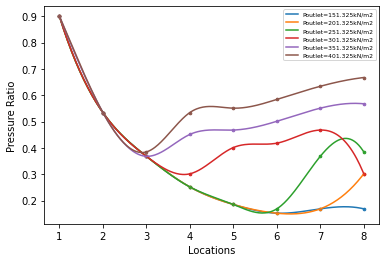
\includegraphics[width=12cm]{figure 1.png}
    \caption{Nozzle A Constant Inlet Pressure Plot}
\end{figure}

    \item \centering {\large Nozzle A: Constant Outlet Pressure 151.325 kN/m2}
     \begin{figure}[!h]
    \centering
    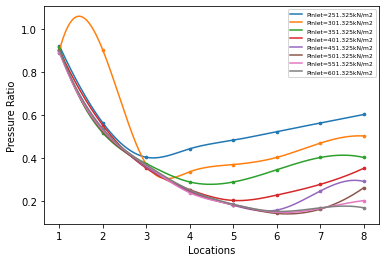
\includegraphics[width=12cm]{figure 2.png}
    \caption{Nozzle A Constant Outlet Pressure Plot}
\end{figure}
\newline
{\tiny Note: Ignore the spike between p1 and p2 at Pinlet=201.325kN/m2 as it was interpreted by spline python for getting an approximate function}

    \item \centering {\large Nozzle B: Constant Inlet Pressure 601.325 kN/m2}
    \begin{figure}[!h]
    \centering
    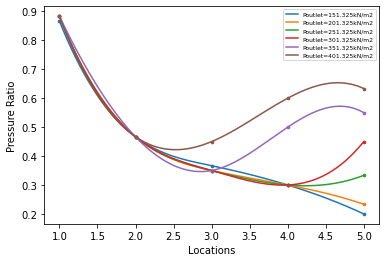
\includegraphics[width=12cm]{figure 3.png}
    \caption{Nozzle B Constant Inlet Pressure Plot}
\end{figure}

    \item \centering {\large Nozzle B: Constant Outlet Pressure 151.325 kN/m2}
    \begin{figure}[!h]
    \centering
    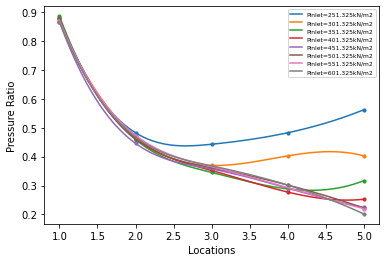
\includegraphics[width=12cm]{figure 4.png}
    \caption{Nozzle B Constant Outlet Pressure Plot}
\end{figure}

\newpage
    \item \centering {\large Nozzle C: Constant Inlet Pressure 601.325 kN/m2}
    \begin{figure}[!h]
    \centering
    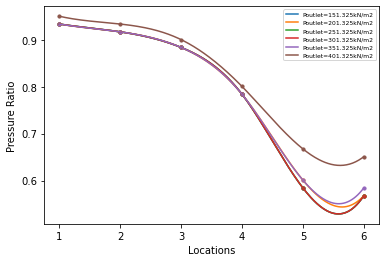
\includegraphics[width=12cm]{figure 5.png}
    \caption{Nozzle C Constant Inlet Pressure Plot}
\end{figure}


    \item \centering {\large Nozzle C: Constant Outlet Pressure 151.325 kN/m2}
    \begin{figure}[!h]
    \centering
    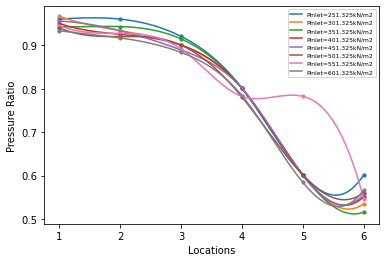
\includegraphics[width=12cm]{figure 6.png}
    \caption{Nozzle C Constant Outlet Pressure Plot}
\end{figure}
\end{itemize}
\newpage

We also need to plot Mass flow Rate wrt to pressure ratios. Snippet of the python code is as follows:
\begin{framed}
\begin{minted}[breaklines]{python}
import numpy as np
import matplotlib.pyplot as plt
from scipy import interpolate

mfr1 =np.array([4.4,4.4,4.4,4.4,4.4,4.4])
pr1=np.array([0.2516526005,0.3348023116,0.4179520226,0.5011017337,
0.5842514447,0.6674011558])
plt.scatter(pr1, mfr1)
x=np.linspace(pr1[0], pr1[-1],300)
k = interpolate.make_interp_spline(pr1, mfr1)
y_new = k(x)
plt.plot(x, y_new)

\end{minted}
\end{framed}

\begin{itemize}
    \item \centering {\large Constant Inlet Pressure 601.325 kN/m2}
    \begin{figure}[!h]
    \centering
    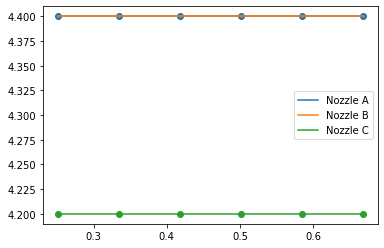
\includegraphics[width=12cm]{figure 7.png}
    \caption{Mass Flow Rate(y-axis) vs Pressure Ratio Plot(x-axis)}
\end{figure}

    \item \centering {\large Constant Outlet Pressure 151.325 kN/m2}
    \begin{figure}[!h]
    \centering
    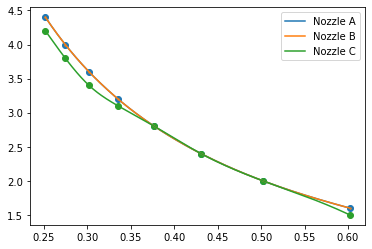
\includegraphics[width=12cm]{figure 8.png}
    \caption{Mass Flow Rate(y-axis) vs Pressure Ratio Plot(x-axis)}
\end{figure}
\end{itemize}




    
